\section[Interfaz gráfica de SuperCollider]{Interfaz gráfica de SuperCollider}
\sectionmark{GUI de SuperCollider}

Cuando instanciamos la clase \texttt{\className}, lo primero que encontramos es una serie de ventanas que se corresponden con los diversos paneles de sintetizador, repartidos a lo largo y ancho de la pantalla del ordenador (fig. \ref{fig:aspecto_SynthiGME}), manteniendo una disposición análoga a la de aquel. Cada ventana tiene como fondo una fotografía del Synthi 100, albergando en su capa superior toda una serie de mandos que provee SuperCollider para el diseño de interfaces gráficas, <<sliders>> y <<knobs>> principalmente. Los colores de estos han sido tomados de la misma fotografía para darle una apariencia lo más integrada posible con el conjunto. 

\begin{figure}
	\centering
	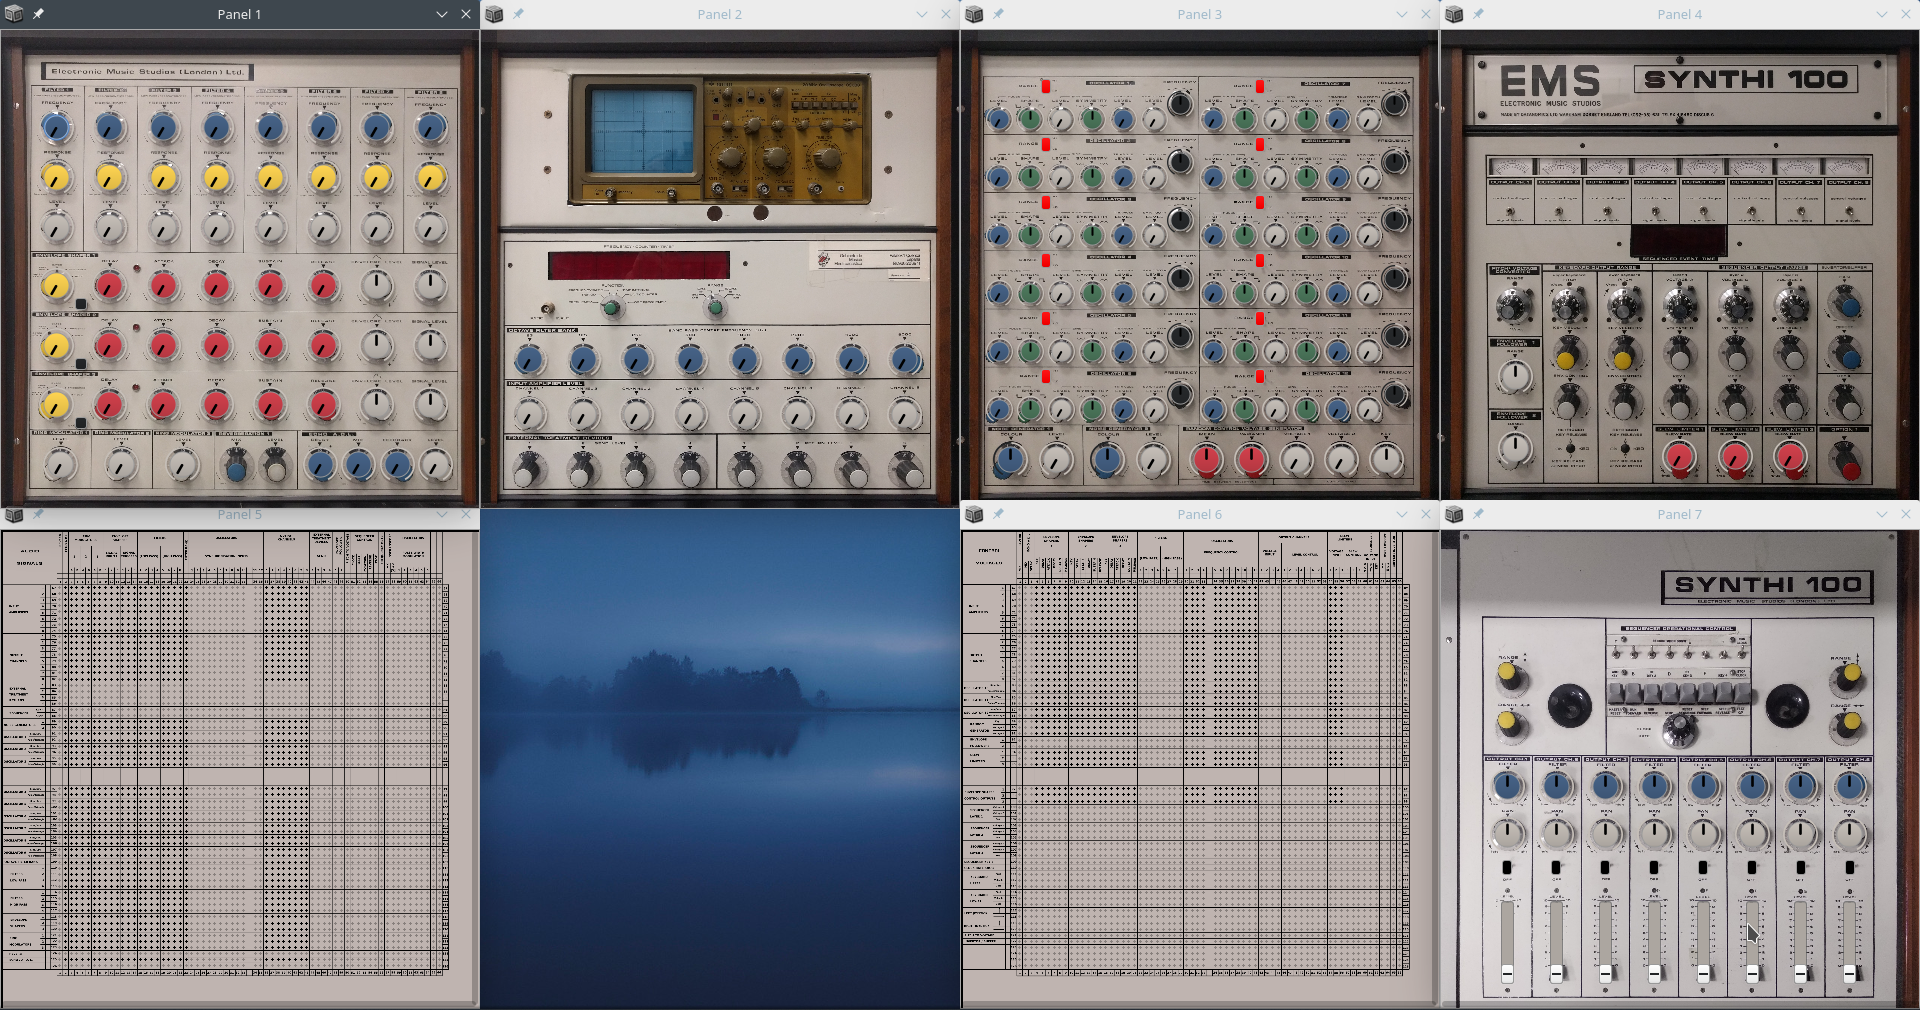
\includegraphics[width=1\textwidth]{images/todos_los_paneles}
	\caption[Ventanas de \appName]{Ventanas de \appName}.
	\label{fig:aspecto_SynthiGME}
\end{figure}
	
Cada una de las ventanas puede ser cambiada de posición y de tamaño de forma independiente. El tamaño por defecto de las ventanas, si bien nos permite tener una visión general del conjunto e identificar rápidamente cada panel del sintetizador, no nos permite ver los detalles suficientes como para trabajar sin hacer zoom. En este punto se hace totalmente necesario cambiar el tamaño de cada ventana sobre la que se desee trabajar. Por esta razón se han creado una serie de atajos de teclado (\textit{cfr.} tabla \ref{table:atajos})  y de ratón para conseguir hacerlo con cierta agilidad. Con un poco de práctica es posible usarlos con mucha soltura tanto en demostraciones como en la creación sonora.
	

\begin{table}
	\begin{center}
		\begin{tabular}{ |l|l| }
  		\hline
  		\texttt{v} & Hace visibles o invisibles los mandos de la ventana en foco\\
  		\texttt{1} & Lleva al frente la ventana del panel 1\\
  		\texttt{2} & Lleva al frente la ventana del panel 2\\
  		\texttt{3} & Lleva al frente la ventana del panel 3\\
  		\texttt{4} & Lleva al frente la ventana del panel 4\\
  		\texttt{5} & Lleva al frente la ventana del panel 5\\
  		\texttt{6} & Lleva al frente la ventana del panel 6\\
  		\texttt{7} & Lleva al frente la ventana del panel 7\\
  		\texttt{e} & Desactiva y activa los pines sin uso en \className\\
  		\texttt{f} & Lleva al frente todas las ventanas\\
  		\texttt{o} & Lleva a al tamaño y posición original la ventana en foco\\
  		\texttt{O} & Lleva a al tamaño y posición original todas las ventanas\\
  		\texttt{+} & Aumenta el tamaño de la ventana en foco\\
  		\texttt{-} & Disminuye el tamaño de la ventana en foco\\
  		\hline
		\end{tabular}
		\caption[Atajos de teclado]{Atajos de teclado de la Interfáz gráfica de Supercollider}
		\label{table:atajos}
	\end{center}
\end{table}

Se ha tenido especial cuidado en usar solo \textit{Views} compartidas por las tres plataformas en las que actualmente se puede compilar SuperCollider (Linux, Windows y MacOS)\footnote{La lista de clases, los frameworks en los que están escritas y su compatibilidad entre plataformas se puede encontrar en la ayuda de SuperCollider: 

\texttt{http://doc.sccode.org/Overviews/GUI-Classes.html} (16 de febrero de 2020) } . Usando exclusivamente estas clases, se garantiza la compatibilidad hacia el futuro del diseño de la interfaz gráfica de usuario.

En cada uno de los diferentes <<widgets>> cuya función es enviar al programa un valor entre un rango continuo ---como es el caso de los diales (<<Knobs>>) y los controles deslizantes (<<Sliders>>)---, podemos variar su valor con diferentes valores de precisión con la ayuda de diversas teclas pulsadas simultáneamente al movimiento del ratón o a la pulsación de las flechas. Ordenados desde el movimiento más grueso al más fino, la teclas a pulsar para alterar la velocidad son: \texttt{Shift}, sin tecla, \texttt{Ctrl} y \texttt{Alt}.

Es importante notar que la forma por defecto en la que se cambia el valor de un dial no es haciendo un gesto rotatorio con el ratón. Se ha optado, en cambio, por un movimiento horizontal. Si bien el movimiento rotatorio puede resultar más intuitivo, tiene la característica que un solo click de ratón sobre el dial cambia su valor de golpe al correspondiente al radio sobre el que el puntero se encuentra. Esto hace imposible hacer click sobre el dial sin alterar su valor drásticamente.